\documentclass[11pt]{article}

\usepackage{amssymb}
\usepackage[english]{babel}
\usepackage{changepage}
\usepackage{cite}
\usepackage{float}
\usepackage[margin=1.5in]{geometry}
\usepackage{graphicx}
\usepackage{lmodern}
\usepackage{setspace}
\usepackage{tabularx}
\usepackage{booktabs}
\usepackage[table,xcdraw]{xcolor}
\usepackage{adjustbox}
\usepackage{url}
\usepackage{listings}
\usepackage{appendix}
\usepackage{caption}
\usepackage{etoolbox}

\usepackage{tikz}
\usetikzlibrary{shapes.geometric, arrows}
\usepackage{standalone}

\usepackage{pgfplots}
\usepgfplotslibrary{statistics}
\usetikzlibrary{pgfplots.statistics}

\usepackage[T1]{fontenc}

\bibliographystyle{ieeetr}

\graphicspath{{figures}}

\newtoggle{label}
\togglefalse{label}


\lstset{
    basicstyle=\small,
    showspaces=false,
    showstringspaces=false,
    tabsize=2,
    title=\lstname,
}

\onehalfspacing

\usepackage{siunitx}
\sisetup{output-exponent-marker=\ensuremath{\mathrm{E}}}

\begin{document}
\pagenumbering{roman}
\thispagestyle{empty}
\begin{center}
\begin{Large}
\emph{Thesis Submitted for Master of Science in Computer Science} \\
Department of Computer Science \\
Rochester Institute of Technology \\
\end{Large}
\vspace{4em}
{\huge A Generalized Model of Cognitive Workload} \\
\vspace{3em}
{\LARGE Taylor Carpenter} \\
{\tt tjc1575@rit.edu} \\
\vspace{3em}
\begin{adjustwidth}{.5in}{.5in}
Chair: Dr. Zack Butler \hfill {\tt zjb@cs.rit.edu} \\
\vspace{2em}
\hrulefill \\
\vspace{3em}
Reader: Dr. Esa Rantanen \hfill {\tt emrgsh@rit.edu} \\
\vspace{2em}
\hrulefill \\
\vspace{3em}
Observer: Sean Strout \hfill {\tt sps@cs.rit.edu} \\
\vspace{2em}
\hrulefill
\end{adjustwidth}
\vspace{2em}
Rochester, NY 14623 USA \\
\vspace{2em}
\today
\end{center}
\pagebreak
\thispagestyle{empty}
\begin{center}
\begin{large}
A Thesis Submitted\\
in\\
Partial Fulfillment of the\\
Requirements for the Degree of\\
Master of Science in Computer Science

\vspace{.5in}

Department of Computer Science\\
B. Thomas Golisano College of Computing and Information Sciences\\
Rochester Institute of Technology\\
Rochester, NY 14623 USA
\end{large}
\end{center}
\pagebreak
\thispagestyle{empty}

\addcontentsline{toc}{section}{Abstract}
\begin{abstract}

\end{abstract}
\clearpage
\section*{Acknowledgement}\addcontentsline{toc}{section}{Acknowledgement}

\clearpage
\tableofcontents
\listoffigures
\listoftables
\pagebreak

\cleardoublepage\pagenumbering{arabic}
\section{Introduction}
Human operators are commonly involved in complex human-machine systems that are present in many industries. With the help of computers and automation, many operators can perform tasks at previously unseen speed and effectivenesses. As such, researchers and engineers have focused on the advancement of the abilities of automation to the point where it is found in a variety of fields. One aspect of automation design that is commonly overlooked however, is the effect it has on the human operator, and thus the overall system effectiveness. Similar to computers, humans have a limited amount of resources that can be dedicated towards a specific task. When the resources are under heavy load, or in the case of a person, when they are overworked mentally, suboptimal decisions and errors can occur. This degradation in performance can lead to serious disasters~\cite{Wickens}. In many cases, it can be difficult to detect the degradation of the operator's effectiveness as primary task performance will be maintained at appropriate levels while secondary tasks receive less attention~\cite{Hockey}. 

Unlike the diagnostic capabilities of a computer system however, methods for monitoring the working state of human operators have not been well developed. The cognitive workload of a person is more difficult to quantify than stress on a computer as the exact workings of the human mind and consciousness are not fully understood. If a system can be developed to monitor the functional state of a person, load balancing methods can be used to transfer work to other human operators, or to autonomous systems through adaptive automation~\cite{Wilson}. Effective, on-line monitoring of cognitive workload could reduce overall system errors and remove unnecessary stress from operators, benefitting both the health of the operator as well as the efficiency of the system. High workload is not the only condition that can lead to errors in a human-machine system. In cases of low workload, operators can become complacent and miss signals that must be addressed due to low vigilance~\cite{Parasuraman}. Thus, an effective cognitive workload monitor must be able to detect multiple levels of cognitive workload.

An effective, generalized model of cognitive workload would reduce the amount of model training required and allow for greatly flexibility as either a larger production system or as a research tool. While a large body of research, {\bf discussed in detail later}, has focused on the generation and effectiveness of specialized, single subject, cognitive workload models, this thesis proposes methodology for generating a cognitive workload model based on psychophysiological data from multiple subjects performing tasks and analyzes the effectiveness and feasibility of the resulting models.

\section{Background}
	\subsection{Terminology}
	The following subsections layout the definitions that are used for various terminology that appear throughout this research. Some of the terms are commonly used in this area of research but have various meanings, depending on the field and background from which the research originates. Other terms are being assigned unique meanings for the purposes of this research. For the sake of clarity, the major terms are explained explicitly, ideally removing confusion on how the terms are being used.
	
		\subsubsection{Cognitive Workload}
		Many definitions exist for ``cognitive workload'', as it is a theoretical concept that is intuitive to understand but difficult to fully encapsulate within a single statement. For the purposes of this research, the definition of cognitive workload is that proposed by Meshkati: ``mental workload [is] a multidimensional construct that reflects the interaction of such elements as task and system demands, operator processing capabilities and effort, subjective performance criteria, operator information processing behavior and strategies, and finally, operator training and prior experience''~\cite{Meshkati}. Since cognitive workload is a theoretical construct, there are no methods of measuring it directly. Instead, loading tasks can be used to affect workload while measurements, such as psychophysiological readings, can be examined that allow for inferences to be made about cognitive workload.  With respect to this research, descriptions for measuring cognitive workload are in fact referring to the indirect measurement of factors affected by workload and making inferences about the underlying load. 
		
		Another term commonly used in the literature is ``operator functional state'' or OFS. The definition of OFS used in this study is that put forth by Hockey: ``the variable capacity of the human operator for effective performance in response to task and environmental demands, and under the constraints imposed by cognitive and physiological processes that control and energize behavior''~\cite{Hockey}. In many applications, such as the current research and various other similar studies, cognitive workload and OFS can be seen as the same construct and used interchangeably. For the sake of clarity, ``cognitive workload'' is the term that is used throughout this research, although studies that are referenced herein may use the term OFS.
		
		\subsubsection{Participant Study}
		Participant study, for the purposes of this research, refers to the data collection process that involved the help of participants. The end result of the participant study was the production of psychophysiological data that was then processed and analyzed as part of the remaining research. 
		
		\subsubsection{Classification System}
		In this research, classification system refers to the processes and Python scripts that acted on the data collected from the participant study. This includes everything from the preprocessing of sensor data to the training and evaluation of classification models. 		
		
		\subsubsection{Model / Classifier}
		Another term that is used throughout this research is ``model''. In this case, the more mathematical definition of model, such as that used in the context of machine learning, is intended, rather than a strictly psychological definition. A model, as used in machine learning, is a system that can take input data and produce some output as defined by patterns present in historical data. These models can be a black-box, which cannot be defined or explained effectively by a person, or they may be described with well defined rules, depending on the technique used. Since the current research deals with the classification of data, the term classifier is also used to refer to the model. It should be noted that ``classifier'', which is the trained model, is distinct from ``classification method'', which is the particular format of the model, such as artificial neural network (ANN).
	
	\subsection{Cognitive Workload Theory}
	
		\begin{enumerate}
			\item What is the theory?
			\item History / When did it come about?
			\item What research has been done?
			\item Are there conflicting ideas?
		\end{enumerate}
	% What is it?
	% Current / previous research into workload

\section{Related Work}
Classifying cognitive workload has been the subject of many studies. The majority of studies have dealt with creating an individual model unique to each participant, with the study consisting of only one task. These studies commonly use EEG and heart rate as psychophysiological features~\cite{Wang_R, Zhang, Wilson, Yang}. While EEG data is consistently used in cognitive workload studies, the subsequent features generated from the data vary. Some of studies, such as the work performed by Wilson et al.~\cite{Wilson}, use log power spectrum information from the EEG measurements while other studies, such as that by Zhang et al.~\cite{Zhang}, use combinations of EEG power spectrum information, called task load indices. In addition to EEG and heart rate, some studies include blink rate~\cite{Wilson, Wilson_2002} and respiration rate~\cite{Wilson_2003} as features. Other studies used blinking and eye movement measures to correct artifacts in EEG data~\cite{Wang_R}. The general layout for each of the studies was roughly the same; participants were attached to a variety of sensors and then asked to perform a loading task at varying difficulty levels to induce different cognitive workloads. The two most common loading tasks used were the Multi-Attribute Task Battery (MATB)~\cite{Comstock} and AutoCAMS~\cite{Lorenz}. These systems are commonly used due to their ability to systematically vary the difficulty settings. 

A variety of classifiers have been used in studies in an attempt to model cognitive workload. The study covered by Yang et al.~\cite{Yang} uses a system of fuzzy inference rules to perform realtime classification of cognitive workload for the purposes of adaptive automation triggering. An SVM Regressor was used by Ke et al.~\cite{Ke} to produce a cognitive workload index, a particular number corresponding to cognitive workload level. Another study~\cite{Wang_R} explored the use of an Adaptive-Network-based Fuzzy Inference System that was trained using differential evolution and ant colony search as a means of predicting levels of cognitive workload. Fuzzy C-Means clustering was used in a study~\cite{Zhang} as a means of classification through clustering. The study completed by Wilson et al.~\cite{Wilson} used an artificial neural network. All of these studies have shown adequate results but have failed to address the larger scope of generalizability. One study~\cite{Wang_Z} used a bayesian model to explore the ability of a model to be used on multiple subjects, learning from and tested on a dataset consisting of data from multiple participants. What the study lacked, however, was the ability to handle novel data; that is, classify on a participant that was previously unseen. A different study~\cite{Ke} falls into a similar category, however it deals with multiple tasks rather than multiple participants. The study involved testing on data from an unseen task,  showing the possibility for full generalization. An additional study~\cite{Christensen} demonstrated how cognitive workload metrics for a single individual can vary substantially across multiple days. This adds an additional challenge to generalizability as the model not only has to account for different subjects and tasks, but also the variation within subjects across multiple days.


\section{Problem Statement}
While many studies have focused on individualized models of cognitive workload using machine learning, few studies have produced results that are of use outside of a controlled lab setting. In a practical application, the training of a model to each individual for every task they may perform would be far too time consuming and costly. This research investigates the effectiveness of a generalized model of cognitive workload based on psychophysiological measures. In order for the model to be generalized, it should be robust against differences between individuals and between the tasks being performed. It should also be effective at handling novel individuals and tasks. Such a model may or may not be reasonably developed due to the complexity of the human mind. Ideally the resulting model could be used outside of a controlled setting with automatic data processing and realtime classification.

A driving factor behind this work is usability in a real-world setting. As such, design decisions were made that favor low-cost, easy-to-use sensors with little to no empirical cleaning of data. The models were trained using the machine learning techniques of artificial neural networks and random forests and tested in a variety of configurations to determine their effectiveness. As is common in this type of study, data for experimentation was collected with sensors from subjects as they participated in cognitive loading tasks of varying difficulties. While no methods used would inhibit realtime analysis, the system focused on offline data.  In the end, this research hopes to address the following hypothesis: a generalized model of cognitive workload that is more effective than random and that can be trained using methods suitable for real-time classification without manual data processing.

	\subsection{Applying Generalized Models of Cognitive Workload}
	A fully generalized model of cognitive workload would be of use in a variety of applications. In some instances it would simply improve on areas where cognitive workload models are already used but in other instances it would open the door to new research.
	
		\subsubsection{Adaptive Automation}
		One application in which cognitive workload models are already used in adaptive automation. Adaptive automation, as described by Byrne and Parasuraman, is automation in which the  ``assignment of tasks between the human operator and automation is dynamically adjusted based on task demands, user capabilities, and total system requirements to promote optimal system performance''~\cite{Byrne}. It has been found in previous studies that static automation, automation that is constant and which puts the operator in a state of monitoring for failures, can result in a deterioration of performance due to the strain of monitoring~\cite{Parasuraman_1993, Parasuraman_1997}. In adaptive automation, through the use of a cognitive workload model, the state of the operator can be monitored and the automation system adjusted accordingly to maintain the desired balance between manual and automatic control. A concept of an adaptive automation system using participant specific cognitive workload models has been done by Wilson, showing improvement in the overall task performance~\cite{Wilson_2005}. The addition of a generalized model of cognitive workload would greatly improve the flexibility of an adaptive automation system as it would eliminate the need for training on each individual user.
		
		\subsubsection{Research}
		While some tasks, such as the Multi-Attribute Task Battery (MATB)~\cite{Comstock} and AutoCAMS~\cite{Lorenz} were specifically developed to have control over the level of the load placed on the user, many other tasks can be much less predictable. Therefore, while it is possible to train individualized models of cognitive workload effectively on specialized laboratory tasks, it is unlikely that the same level of training could occur with more complicated tasks that are reflective of other real-world situations. In many cases, knowledge gained while studying one situation or task is used to make predictions and assumptions about another domain. It has been noted, however, that special care must be taken when dealing with analogous systems as the situations could be more different than they seem due to underlying complexity~\cite{Huey}. If a generalized model of cognitive workload were created that was effective independent of task, it could be trained on the specialized loading tasks, such as MATB, and then used in other domains to better research the workload of tasks, without the need for analogous systems and the danger of faulty comparisons.


\section{Participant Study}
A study was conducted in order to generate and collect the data needed to train the appropriate models and to test the underlying concept of developing a generalized model. While previous research~\cite{Wang_Z} has relied on the use of established and validated data collected from other experiments~\cite{Wilson_2010}, the amount of data required to adequately train artificial neural networks was not available. Consequently, a new study was required to generate the large amount of data that was necessary. The participant study consisted of two tasks, each with a leading baseline trial and three load conditions. The load condition trials were ten minutes long and the baseline trials were five minutes long. 
The initial design of the participant study specified fifteen minute long trials but feedback from the pilot group suggested that at fifteen minutes, task fatigue started affecting performance.

The participant study began with a total of ten college-aged participants, similar to existing studies~\cite{Ting,Wang_R,Wilson_2010, Yin, Zhang}, however, due to complications, only seven participants completed the entire process. 
Two of the removed participants were excluded due to an improperly fitted EEG headset as well as discrepancies between the task difficulties reported versus the average difficulties reported by the other participants. The last removed participant was excluded due to personal issues preventing the completion of the tasks. Additionally, one of the remaining seven participants completed only one trial of the low-workload RanTask condition, rather than the intended two trials, due to sensor and software issues.

Of the seven participants that completed the participant study, the ages ranged from 18 to 23 years old, with an average age of 21.1 years. The gender ratio was balanced with three males and four females. Participants lacked any uncorrected hearing or visual impairments that would affect performance on the tasks of the study. 
The following subsections describe each of the tasks as well as the overall layout of the participant study in its entirety.
	
	\subsection{Multi-Attribute Task Battery (MATB)}
	The first loading task presented to participants was the Multi-Attribute Task Battery (MATB), a task loading system originally developed by NASA~\cite{Comstock}. MATB is a system that has been used in a variety of studies as a means of task loading for the collection of psychophysiological data~\cite{Wilson, Smith, Wang_Z}. The system consists of a multitude of subtasks arranged in such a way as to simulate the tasks a pilot might be required to perform during flight. The particular version of the system used in this study was AF-MATB, an updated version of the original software~\cite{Estepp}. This version is very similar to the original with the majority of the changes affecting how it runs on modern operating systems and adding different options for subtask automation. All of the subtasks of MATB were used in the study, while the scheduling view that shows upcoming events was disabled. Input to the system was in the form of joystick and either keyboard or mouse. Participants were free to decide whether to use the keyboard, mouse, or a combination of the two with the right hand while the joystick was controlled with the left hand. In Figure~\ref{fig:matb}, the main view of MATB with which participants interacted is shown. This includes resource management, systems monitoring, communications, and tracking. 
	
	\begin{figure}[]
	\centering
	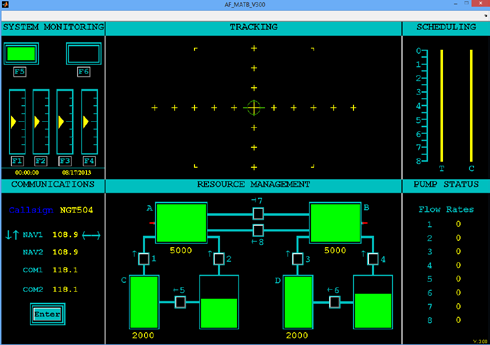
\includegraphics[width=\linewidth]{figures/matb.png}
	\caption[Multi-Attribute Task Battery (MATB) Main View]{Main view of the MATB simulation software. }
	\label{fig:matb}
	\end{figure}
	
	The resource management subtask involved maintaining the amount of fuel that was present in two main tanks within a small acceptable range. Secondary tanks were present and could be used to temporarily store fuel. The participant was required to toggle pumps, controlling the flow of fuel between the tanks. Throughout the trial, pumps would temporarily break, or silently shut-off, preventing the flow of fuel through the pump. The number and frequency of these occurrences depended on the difficulty condition of the trial.
	
	The systems monitoring subtask were centered around two buttons and four gauges. One button was to be kept on while the other button was to be kept off. Throughout the simulation, the buttons changed states and the participant was required to click on the button indicator, or press a corresponding key, to revert the button to the correct state. Colors were used to indicate the state of the buttons. Background color indicated that the button was off, while either red, for the ``off'' button, or green, for the ``on'' button, was used to indicate on. The gauges presented had sliders that would vary in vertical position throughout the simulation. Occasionally, depending on the difficulty condition, a slider would move outside the acceptable range for the gauge and require interaction from the participant, either through a mouse click or key press, to reset the gauge. If an out-of-state system component was not addressed within the response time period of ten seconds, the component was automatically reset to its defaults, within-range state.
	
	The communication subtask required the use of sound. The participant was assigned a particular aircraft callsign. For the duration of the trial, the participant was required to listen for their callsign and respond to the instructions. The communication window included four different communication channels, each set to a particular frequency. Throughout the simulation, recorded audio tracks would play, addressing a particular callsign to change a channel to a desired frequency. If the callsign matched that of the participant, they were to change the specified communication channel to the appropriate frequency using either the mouse or the arrow keys. If the callsign did not match that of the participant, the request was to be ignored. The number and rate of true- and false-alarm requests depended on the difficulty condition of the trial.
	
	The tracking subtask was the only one that required the use of the joystick. The participant simulated steering a plane by keeping a reticle within the acceptable parameters of the tracking window. The amount of drift affecting the reticle and the amount of control the joystick emitted onto the reticle varied throughout the simulation in accordance with the difficulty condition of the trial. 
	
	\begin{table}[]
	\centering
	\caption[Multi-Attribute Task Battery (MATB) Load Condition Parameters]{Parameters used in MATB script generator specifying subtask difficulty and event occurrences per 10-minute trial}
	\adjustbox{max width=\textwidth}{
	\begin{tabular}{llllllll}
	\toprule
	\rowcolor[HTML]{FFFFFF} 
	 &  & \multicolumn{2}{c}{\cellcolor[HTML]{FFFFFF}Communication} & \multicolumn{2}{c}{\cellcolor[HTML]{FFFFFF}System} & \multicolumn{2}{c}{\cellcolor[HTML]{FFFFFF}Resources} \\ \cmidrule(l){3-8} 
	\rowcolor[HTML]{FFFFFF} 
	Load Condition & Tracking & Target & Distractor & Lights & Gauges & Failures & Shut-offs \\ \midrule
	\rowcolor[HTML]{EFEFEF} 
	Low & Low & 6 & 2 & 48 & 42 & 4 & 2 \\
	\rowcolor[HTML]{FFFFFF} 
	Moderate & Moderate & 18 & 10 & 96 & 102 & 20 & 10 \\
	\rowcolor[HTML]{EFEFEF} 
	High & High & 30 & 12 & 110 & 120 & 40 & 20 \\ \bottomrule
	\end{tabular}
	}
	
	\label{tab:matb-params}
	\end{table}
	
	The baseline condition for MATB involved the participant watching the screen while the simulation ran with the low condition parameters and automation of all available tasks enabled. This allowed for the visual and auditory stimulation without the cognitive workload. Presented in Table~\ref{tab:matb-params} are the parameter values that were entered into the script generator of MATB to produce the trials for each load condition. Each parameter, with the exception of tracking difficulty, represents a type of event that can occur during the simulation. The value for a parameter specifies how many times the event should occur over the length of the 10-minute trial. Two scripts were generated for each difficulty condition to ensure that each trial was different and the participants could not memorize any patterns. The parameter values used are based off those in a previous study ~\cite{Estepp_2015}. The majority of the parameter values are scaled from the referenced values to account for the difference in trial lengths, however the parameters for ``lights'' and ``gauges'' in the high condition were further modified due to errors in scheduling from the script generator. 
	
	
	\subsection{RanTask}
	The second loading task used in this study is a custom tone counting task, referred to herein as RanTask. This task is an extension of the mental workload loading task used in the work of Rantanen et al.~\cite{Rantanen}. The participant was presented with three different tones in a random order. The participant was to count the tones that were presented and press the key corresponding to the tone when the desired count was reached. The intended count differed with the difficulty condition. The tones corresponded to the notes B at 493 Hz, F at 698 Hz, and A at 880 Hz. Each tone was presented for one second with a one second interval between tones, giving the participant two seconds to respond to a given tone. Each time a tone was presented, a log entry was created, recording the tone presented, its number in the sequence, and whether, if a participant pressed a key, it was correct or incorrect. If a key was pressed at an incorrect time, a false-positive was logged and the sequence count for the corresponding tone was reset to prevent cascading failure, e.g. counting every five correctly but being off by one from the ground truth sequence would result in all false-positive without the reset. 
	
	\begin{table}[]
	\centering
	\caption[RanTask Load Condition Tone Counts]{RanTask Desired Tone Counts}
	
	\adjustbox{max width=\textwidth}{
	\begin{tabular}{llll}
	\toprule
	\rowcolor[HTML]{FFFFFF} 
	 & \multicolumn{3}{c}{\cellcolor[HTML]{FFFFFF}Tone Frequency} \\ \cmidrule(l){2-4} 
	\rowcolor[HTML]{FFFFFF} 
	Load Condition & Low & Moderate & High \\ \midrule
	\rowcolor[HTML]{EFEFEF} 
	Low & 0 & 5 & 0 \\
	\rowcolor[HTML]{FFFFFF} 
	Moderate & 2 & 0 & 3 \\
	\rowcolor[HTML]{EFEFEF} 
	High & 2 & 2 & 3 \\ \bottomrule
	\end{tabular}
	}
	
	\label{tab:rantask-params}
	\end{table}
	
	In the baseline trial, the participant was not required to count any of the tones, only listen. Presented in Table~\ref{tab:rantask-params} are the desired counts for each tone in each load condition. This differs from the originally intended counts due to feedback from the pilot study members. Feedback indicated that the original low- and moderate-load conditions, both requiring the counting of a single tone, were too similar in difficulty. As such, the moderate-load condition was replaced with the existing high-load condition and an additional condition was added that required keeping count of all three tones. The participants were given a copy of the count information from Table~\ref{tab:rantask-params} at the time of the trial to ensure they were aware of which tones were to be counted. The participants were also informed that the use of fingers for counting or any other external methods of keeping track of tones was prohibited.
	
	\subsection{NASA Task Load Index (TLX)}
	The NASA Task Load Index (TLX) assessment is a means of determining the workload for a given task subjectively based on participant responses~\cite{NASA}. The procedure allows for exploring the different aspects of a task and where the underlying cognitive workload originates. The workload rating obtained from participants through the TLX process was used to compare the subjective difficulties of the various tasks, similar to the procedure used in existing studies~\cite{Ke, Estepp_2015}. The current TLX procedure consists of six subscales: Mental Demands, Physical Demands, Temporal Demands, Own Performance, Effort, and Frustration. The Mental Demands subscale measures how much mental activity was required and its complexity. Physical Demands measures how much physical activity was required and how laborious it was. Temporal Demands measures how much time pressure was present in the task. In the Own Performance subscale, the participant remarks on how successful they felt they were and how satisfied they are with their performance. The Effort subscale measures how hard the participant had to work to accomplish the task. The final subscale, Frustration, measures how stressed or relaxed the participant felt during the task. 
	
	Individual calibration was required from each participant for both of the tasks that were performed. During this calibration, the participant performed pair-wise comparisons between the TLX subscales, indicating which subscales had more effect on the overall workload of the task. The calibration was then used as a method of weighting the individual TLX survey responses for a trial. The idea behind the weighting is that a component that is calibrated as having a large impact on the overall workload should have its rating affect the overall workload metric more heavily. The overall TLX index was used for each participant, that is the sum of the weighted subscale components.
		
	\subsection{Study Execution}
	The participant study took place over four days for each participant. Each day required roughly an hour and a half from the participant. The time was approximate as it was dependent on how quickly the sensors were placed which was, at times, delayed due to obstructions, e.g. hair. The first day consisted of an introduction to the system: what sensors were to be utilized, the intent of the study, and what was to be expected of the participant. Additionally, each participant signed an informed consent form after being fully briefed on what the study entailed. Training was also conducted on each task to familiarize the participant with what was to be expected. Ideally, stable performance on both tasks was achieved for all participants as a result of training. Other studies~\cite{Wilson} have included lengthier training periods however, due to time constraints, the time required for complete stability was not feasible. 
	As such, the task performance results of each participant were recorded and examined as a factor in the overall effectiveness of this study. 
		
	The second day marked the beginning of data collection for the participants. The participants were attached to the sensors and a five minute baseline recording using MATB was taken. Following the baseline, the participants each completed a ten minute MATB trial on the low-load condition. A NASA-TLX survey was then administered to record the participants' rating of the task workload. Next, the participants completed a second, ten minute MATB trial on the low-load condition. This again was followed by a NASA-TLX survey. Two TLX surveys were taken for each condition to evaluate the stability of the rating as participants should be recording similar ratings for both trials of a condition. After a ten minute break, the same procedure was repeated, including the baseline, substituting RanTask for MATB as the task being performed.
	
	The third and fourth days followed the same format as the second day. The third day consisted of the tasks being performed on the moderate-load condition while the fourth day consisted of the tasks being performed on the high-load condition. Each participant performed all their trials at similar times of day to reduce variations caused by circadian rhythm. The order in which the load conditions were presented follows that of a previous study~\cite{Wilson}. While the sensors were removed and replaced on multiple occasions as the data collection occurred over many days, which differs from some studies~\cite{Wilson, Ke, Zhang}, this should not have an effect on the overall validity of the data~\cite{Estepp_2015}.


\section{Application of the Classification System}
The classification system that was created encompassed a full classification workflow. It covered the collection of data from the sensors, preprocessing to restructure the data into a more usable format, processing to generate features, training of classifiers, and evaluating the classifiers with the appropriate datasets. The system is modular, such that each task can be performed individually, allowing for flexibility with future extensions of functionality. 
In Figure~\ref{fig:system-overview} an overview of the entire classification system is shown. In the following subsections, the various components of the system will be discussed in detail. 
\begin{figure}
\centering
\adjustbox{max width=\textwidth}{
\includestandalone{figures/system_overview}
}
\caption[General Overview of Complete Classification System Workflow]{A general overview of the entire classification system workflow.}
\label{fig:system-overview}
\end{figure} 

	\subsection{Sensors}
	Data was collected through the use of two sensors, an EEG monitor and a heart rate monitor. The collection of psychophysiological data through EEG and heart rate monitors has been performed in numerous existing studies~\cite{Wilson, Yang, Wang_Z} and has been assessed and found to be valid~\cite{Sweller}. Following with the theme of practicality in a production system, the sensors used are more readily available than those used in other research settings. Data collection was structured such that there was one heart rate data file and one EEG data file per trial period, as opposed to recording multiple trials in a single file. As such, the data recording process was started shortly before and stopped shortly after each trial, resulting in a small amount of extraneous, noisy data preceding and trailing the trial data.
		
		\subsubsection{Electroencephalogram (EEG)}
		The electroencephalogram (EEG) monitor used is a wet-contact, wireless headset called the Emotiv EPOC+~\footnote{Emotiv EPOC+ product details available at \url{https://emotiv.com/epoc.php}}. The EEG monitor is a research grade headset with 14 individual data channels and two reference channels. Electrodes on the headset were located at the following placement sites as defined by the International 10-20 System for electrode placement~\cite{Jasper}: AF3, F7, F3, FC5, T7, P7, O1, O2, P8, T8, FC6, F4, F8, and AF4. Electrodes placed at P3 and P4 served as references for the headset. The predecessor to this headset, which is very similar to the current headset, has been proven effective in many studies including work by Knoll et al.~\cite{Knoll}. The design of the headset allows for accurate placement of electrodes over many trials and does not need an expert for proper setup due to the presence of rubber guides that are placed on the mastoids of the participant. The use of a headset as opposed to stand-alone electrode contacts does lead to some issues regarding proper scalp contact with individuals having smaller-than-average skulls or large amounts of hair. Data collection software for the EEG headset allowed for monitoring of contact quality of the electrodes, ensuring proper readings were taken. Thanks to the work done by Estepp et al.~\cite{Estepp_2015}, it can be assured that the removal and replacement of electrodes between data collection trials had little to no effect on the quality of the measurements. The headset operates at a resolution of 128 samples per second. This high resolution resulted in more data and reduced the amount of variation caused by instantaneous noise.
			
		\subsubsection{Heart Rate (HR)}
		The heart rate monitor used was an optical, arm-based monitor called RHYTHM+ by Scosche~\footnote{RHYTHM+ product details available at \url{http://www.scosche.com/rhythm+}}. The monitor was designed for collection of vitals during fitness training, not research, but it was sufficient for the monitoring of participants. At a resolution of four samples per second, much less data was collected for heart rate than EEG. This was not an issue, however, as heart rate change is gradual and unlikely to vary rapidly. An arm-based monitor was chosen as it was more comfortable and convenient to participants than a chest-strap monitor. The monitor communicated with the data recording computer through a protocol called ANT~\footnote{Additional information on the ANT protocol can be found at \url{http://www.thisisant.com}}, a protocol commonly used within fitness equipment.  The monitor can easily be adjusted and was unobtrusive enough to be worn for extended periods of time.
		
	\subsection{Data Preprocessing}
	The preprocessing of data files was necessary to transform the data logged from the sensors into a form that was more easily used to produce features. Rather than modifying the format in which the sensors logged the data, this step was used to extract the information useful for feature generation and write it out to multiple files. This step also encompassed cleaning of the data, addressing issues caused by communication between the sensors and receivers. Each participant trial was preprocessed independently and required no information that was not already contained within the trial data. The majority of the preprocessing for heart rate and EEG data was separate, as is described in the following two subsections, however, once the data had been cleaned, joint processing was required to properly align the times of the two datasets. As mentioned previously, the data files included leading and trailing noise that was not collected during the trial period itself. This data needed to be removed as it was not obtained under the load conditions and had no appropriate label. Part of the information that was logged during task trials was the start time of the trial. This time was used as a starting point when looking for a timestamp on the heart rate data that matched a timestamp in the EEG data. Once a time was found in which EEG and heart rate data existed that was after the start time of the trial, five-second intervals of data were taken until ten-minutes, the length of a trial, of data was processed. This not only removed the leading and trailing noise, it also synchronized the timing between the heart rate and EEG data so that the first five-second interval in the heart rate data corresponded to the first interval in the EEG data.
	
	The data was split into intervals in an attempt to reduce the effect of noise. The use of segmentation is common when dealing with psychophysiological data with a variety of segmentation conditions having been used in previous studies, ranging from two-second intervals with no overlap~\cite{Smith} to 40-second intervals with 35-seconds of overlap~\cite{Wang_Z}. An interval length of five-seconds, a length that has been used in a previous study~\cite{Yin}, was chosen as it is long enough to benefit from averaging and noise reduction but short enough that updates to the participant state are useful to other systems in an on-line manner. 
	
		\subsubsection{EEG}
		The preprocessing of the EEG data involved multiple steps to transform the data from a single EDF file into multiple, separate channel text files. The process that was followed is outlined in Figure~\ref{fig:eeg-preprocessing}. The first step using EEGLAB~\cite{EEGLAB}, an open-source MATLAB toolbox for processing EEG signals, was to read the information out of the EDF file created by the sensor logging and to separate the individual channel streams. A baseline removal process was performed using EEGLAB on each channel, where the baseline of a channel was defined as the mean value of the channel for the time period. Once the baseline was removed, each channel was written out to its own intermediate, tab-separated text file. The channel data was then partitioned into five-second intervals in the method previously described such that each interval fell within the time frame of the trial and aligned with the heart rate intervals. Each channel is then, once again, written out to its own tab-separated text file. The advantage of multiple, intermediate text files is that modifications can be made to later portions of the workflow and applied without a complete reevaluation of earlier steps.

		\begin{figure}
		\centering
		\adjustbox{max width=\textwidth}{
		\includestandalone{figures/eeg_preprocessing}
		}
		\caption[Overview of EEG Preprocessing Workflow]{An overview of the steps involved in the EEG preprocessing workflow.}
		\label{fig:eeg-preprocessing}
		\end{figure} 
			
		\subsubsection{Heart Rate}
		The recorded heart rate data required less preprocessing than the EEG data due to it being only a single channel. In Figure~\ref{fig:heart-preprocessing}, the overall process followed is shown. Once the data was read in, it was smoothed to ensure there was at least one data point per second. While ideally there would be multiple heart rate samples per second, issues in communication between the sensor and the receiver resulted in some periods of time in which no readings were recorded.  Since heart rate undergoes gradual change, missing data points were interpolated from the previous and following heart rate readings.  After the data was smoothed, the heart rate records were partitioned into five-second intervals, as previously described, and written to a tab-separated text file.  

		\begin{figure}
		\centering
		\adjustbox{max width=\textwidth}{
		\includestandalone{figures/hr_preprocessing}
		}
		\caption{Overview of the heart rate preprocessing workflow.}
		\label{fig:heart-preprocessing}
		\end{figure} 
			
	\subsection{Data Processing and Features}
	Data processing to produce the desired features was done after the heart rate and EEG data had been cleaned and preprocessed. A total of 72 features were generated for each five-second interval. Of the 72 features, 70 were EEG features, coming from five spectral bands on each of the fourteen channels, and two were heart rate features. Figure~\ref{fig:feature_generation} presents an overview of the processing steps that changed the preprocessed data into a collection of feature vectors. In addition to the feature values, each feature vector record was labeled with a class value corresponding to the load-condition of the trial from which the data originated, either low, moderate, or high. The data for each task of a participant, at this point labeled with the appropriate class, was combined together such that it could be handled more easily by the classifiers. Data records of each task for each participant were kept separate to ensure the appropriate training and testing datasets could be created during the classifier phase.

	\begin{figure}
	\centering
	\adjustbox{max width=\textwidth}{
	\includestandalone{figures/processing}
	}
	\caption{Overview of the processing and feature generation workflow.}
	\label{fig:feature_generation}
	\end{figure} 
	
		\subsubsection{EEG}
		The end goal of processing the EEG data was the production of band information resulting from the spectral power analysis of each channel.  The processing and feature generation was performed on each channel independently before the features were joined together into one record. The features for a channel were created through the application of a Fast Fourier Transform on each five-second interval of data using a MATLAB function. This transform produced power spectrum information of the EEG channel for the time interval. The bands used as features consisted of delta (1-3 Hz), theta (4-7 Hz), alpha (8-13 Hz), beta (14-30 Hz), and gamma (31-42 Hz). These are the same bands that were used in the work done by Wilson et al.~\cite{Wilson}, as well as various other studies~\cite{Estepp_2015, Christensen}. The band values were computed by summing the logarithm of the power spectrum values that corresponded to the frequencies in each band. The logarithm of the values was taken to normalize the numbers. The five band values for each channel were then combined to produce the complete vector of 70 EEG features. It is important to note that no empirical noise reduction or artifact correction was done between the collection of EEG data and the creation of the features. While this modification would likely increase the effectiveness of the models and is indeed done in many other studies~\cite{Estepp_2015,Ting, Smith}, the driving factor behind this study was to have a system feasible for production, and an expert will not always be available to hand filter the data in a live system. 
			
		\subsubsection{Heart Rate}
		The heart rate data contributed only two features to the overall feature vector. Before any features were generated, however, the mean heart rate of the baseline trial was subtracted from every data point. The idea is that each participant likely has a different resting heart rate; removing the mean of the base heart rate will create offset readings that are caused by the load of the trial. Since removing the mean heart rate could potentially create non-positive numbers and complicate further computations, a constant offset was added across all participants. This shift factor did not affect any patterns that may exist in the data but prevented calculation errors such as divide-by-zero. The first feature to be created from this modified data was the mean heart rate for each five-second interval. The second feature used was heart rate variation or HRV, the ratio between the standard deviation and mean of heart rate for the five-second time interval, similar to that used by Zhang et al.~\cite{Zhang}: \[HRV = \frac{\theta_{HRV}}{\mu_{HRV}}\] where \( \theta_{HRV} \) is the standard deviation and \( \mu_{HRV}\) is the mean of the HR data for a particular time segment.
				
		
	\subsection{Configurations}
	The feature vectors generated from the psychophysiological data was combined in a variety of ways to create different training and test dataset configurations. While the end goal was a model that was both participant- and task-independent, a number of benchmarks along the way provided additional information on the models' generalizability. Each component of a configuration has three possibilities: same, all, and cross. `Same' refers to being trained and tested on the same individual or task. This setting serves as a control, preventing the component from affecting the generalization. `All' refers to combining all the data from the participants or tasks to create both the training and test datasets. This setting explores the classifiers' ability to differentiate between the individual patterns or create a single pattern that is representative of all the participants or tasks. `Cross' refers to training on a subset of the participants or tasks and testing on the remaining participant or task. This setting is the end goal of generalizability as it allows the model to be trained with a specified dataset and then used with a variety of novel participants and tasks. All training and testing dataset splits were stratified with respect to load condition to ensure models could be adequately trained. Additionally, in any situation where both training and testing datasets were created from the same data, as is the case with `same' and `all' configurations, three-fold cross validation was used to ensure results were not dependent on anomalies in the specific data split.
	
	The following subsections described each of the configurations that were utilized in more detail. For convenience, a naming system in the style of acronyms has been created for referencing particular configurations; e.g. ``SP-ST'' refers to ``Same Participant - Same Task''.
		
		\subsubsection{Same Participant - Same Task (SP-ST)}
		Each classifier was first trained and evaluated in a manner similar to previous studies~\cite{Wilson, Zhang, Wang_R, Yin}. This served as a baseline to compare the overall performance of the models to those created in other studies. The main use of this configuration was in determining the effectiveness of the created features. As part of this configuration, the data for each participant on each task was used for both training and testing. This means the classifier was dependent on both the participant and the task. This configuration involved 14 classifiers per classification method, one for each task for each person.
		 
		\subsubsection{All Participants - Same Task (AP-ST)}
		One step up in generalizability is the creation of a classifier that is trained on multiple subjects, similar to that of a previous study~\cite{Wang_Z}. The data for each participant for each task was split into training and testing subsets. The training and testing subsets for all participants on a particular task were then combined to create joint datasets. This explored the possibility of finding patterns in the data that match multiple participants, as opposed to a unique pattern for each participant. This configuration involved two classifiers per classification method, one for each task.
		
		\subsubsection{Same Participant - All Tasks (SP-AT)}
		Another configuration that was explored is similar to the previous configuration, All Participant - Same Task, except the task data was merged, rather than the participant data. The configuration started the same way as the previous two configurations, with the data of each task for each participant being split into training and testing subsets. Then, the training and testing datasets for each task for a participant were combined. A total of seven classifiers for each classification method were trained for this configuration. This explored finding patterns that exist between the tasks, given a particular participant.
		
		\subsubsection{All Participants - All Tasks (AP-AT)}
		The configuration of combined participants and combined tasks is another step up in generalizability. This configuration is a combination of the previous two configurations. In this configuration, all the data was split into training and testing subsets which were then combined across all participants and all tests. The models trained from this configuration explored increased generalizability over existing studies but did not explore the model's capabilities with completely novel data. Only a single classifier per classification method was necessary for this condition.
		
		\subsubsection{Cross Participant - Same Task (CP-ST)}
		This configuration is the first that deals with true generalizability. For this configuration, the data for six of the participants for each of the tasks was combined to form the training set. The last participant served as the test set. Rather than differentiating between patterns previously seen, as the All Participants - Same Task configuration does, this configuration explored how well the patterns learned for a set of participants can generalize to novel data that may contain a distinct, and previously unseen pattern. This configuration resulted in 14 classifiers for each classification method, accounting for the two different task datasets and each participant being the unseen test data for a model.
		
		\subsubsection{Same Participant - Cross Task (SP-CT)}
		Another configuration that was explored is a variation of the previous configuration, substituting participant crossing with task crossing. In this configuration, each classifier was trained on the data for one task for a participant and tested of the data for the second task. This classifier explored how well the patterns discovered in one task generalize to a separate, unseen task. A total of 14 classifiers per classification method were created, allowing for each task to be the test data.
		
		\subsubsection{All Participant - Cross Task (AP-CT)}
		One step down from complete generalization involves combining the previously described options, `all' and `cross'. This configuration involved combining the data for all participants, resulting in one dataset for each task. A single classifier was then created that was trained on the data for one task and tested on the second task. This configuration is similar to the previous configuration, but rather than a unique classifier for each participant, only one was created. This configuration is similar to a previous study~\cite{Ke}. This explored the possibility of a general pattern being found for cognitive workload that can be used independent of task. The configuration resulted in two models per classification method.
		
		\subsubsection{Cross Participant - All Tasks (CP-AT)}
		This configuration is similar to the previous configuration, however it explored the independence of participants instead of tasks. The configuration involved combining data for all tasks, resulting in seven datasets, one for each participant that included both tasks. A classifier was then trained on the data from six participant and tested on the last participant. After repeating the configuration, to test on each participant, a total of 14 models were created.
		
		\subsubsection{Cross Participant - Cross Task (CP-CT)}
		The final configuration represents complete generalizability. It explored the independence of both the participant and the task at the same time. The setup for this configuration involved training a classifier on the data of one task for six participants. The classifier was then tested on the data for the last participant performing the other task. To achieve full test coverage, this condition was repeated 14 times; once for each participant / task test combination.
		
		\subsubsection{Overview}
		A large number of models were created to test different configurations of training and testing data. Table~\ref{tab:configuration} displays how many models were created for each configuration as well as the total number of models created. The table only shows the number of final models, during the training and tuning process many more models were created, evaluated, and discarded due to suboptimal accuracy rates. The table also only shows the number of models per classification method, the actual number of final models is twice what is shown in the table due to two classifier methods being evaluated.
		
		\begin{table}[]
		\centering
		\caption[Configuration Model Counts]{Model Count Per Configuration}
		\adjustbox{max width=\textwidth}{
		\begin{tabular}{@{}lcccccccccc@{}}
		\toprule
		\multicolumn{1}{c}{} & SP-ST & AP-ST & SP-AT & AP-AT & CP-ST & SP-CT & AP-CT & CP-AT & CP-CP & Total \\ \midrule
		\begin{tabular}[c]{@{}l@{}}Number \\ of  models\end{tabular} & 14 & 2 & 7 & 1 & 14 & 14 & 2 & 7 & 14 & 75 \\ \bottomrule
		\end{tabular}
		}
		\label{tab:configuration}
		\end{table}
		
	\subsection{Classifiers}
	Two classification methods were used in the training and evaluation of models, artificial neural networks and random forests. During the training process, a grid search was used to evaluate various combinations of input parameters and tune the model. This tuning occurred for each final model that was created, rather than at a configuration level; e.g. for the 14 models required for the SP-ST configuration, the tuning process was repeated 14 times. Therefore optimal parameters for one model in a configuration are not necessarily consistent with the optimal parameters of another model in the same configuration. This process was automated, using the classification accuracy to determine which model was most effective, and no manual analysis of the tuning results was required. As such, the tuning is still viable for a real-world classification system . The classification accuracy was used in determining which of the created models was most effective for a dataset.  The following subsections detail what libraries were used in the creation of models as well as what parameters were used. 

		\subsubsection{Random Forest}
		Ensemble classification methods, such as random forest, are not common in previous studies of this kind, even though they perform at least as well as other types of classifiers in most situations.The Scikit-Learn~\cite{Scikit} Python library was used for the training of random forest models as it is easy-to-use and is parallelized effectively. Two input parameters were tuned in the training of the models: tree depth and number of trees. There are many other parameters that could have been tuned but they have less of an effect on the overall accuracy and each additional parameter being tuned would have greatly increased the number of models to be trained and evaluated. The number of trees was varied across the following values: 50, 100, 150, 300, 500, 750, 1000, 1500, and 2000. The number of trees controlled how many individual decision trees were present in the random forest model and allowed to vote for a classification. The more trees in a model, the more accurate the approximation of the sample space and any patterns that are contained within, however too many trees leads to a large training time and possible overfitting to the training data. The second parameter that was tuned was max tree depth, which was varied across the following values: 50, 100, 200, 300, 400, 500, 600, 700, and 800. This parameter controls how deep an individual tree in the model can go, i.e. how many branch points a tree can have. Too few branches leads to the decisions being made without looking at enough information but too many branches and the model becomes either overfit to the training data or reliant on features that do not affect the classification. All other parameters that were not actively tuned were kept at the default values as defined by the Scikit-Learn library.
		
		\subsubsection{Artificial Neural Network (ANN)}
		Artificial neural networks (ANN) have been proven in previous studies~\cite{Wilson, Estepp_2015} to be successful in classifying cognitive workload levels of single participants. As part of this study, this classification technique is now expanded to evaluate how effective it is at a generalized model. The ANN library used was the Fast Artificial Neural Network (FANN)~\cite{FANN} library with Python bindings. The library handled all components of the ANN model, from training and parameter setting to evaluation. As the training of ANN models is able to be parallelized easily, multiple models were trained simultaneously, each model training on a single core. This, as well as the nature of ANN training, resulted in models that took far longer to train than the corresponding random forest models.
		
		Artificial neural networks have a large number of parameters that can be changed to achieve different results. Due to the already lengthy amount of time required to train an ANN, the number of parameters that were tuned was kept to a minimum. A three layer neural network was used, having only a single hidden layer. The input layer contained 72 nodes, corresponding to the 72 features in the feature vectors. The output layer contained three nodes, each node representing one of the possible load condition classes. The number of nodes in the hidden layer was tuned from the following values: 72, 60, and 40. Another parameter that was tuned was the connection rate between the nodes. Connection rates of 0.7, 0.9, and 1.0 were evaluated. The last parameter that was tuned was the desired error rate. In the initial configurations, values of 0.01, 0.001, and 0.0005 were evaluated, however this was removed and a value of 0.01 was used for the later configurations as the training time was high and none of the models were able to reach the desired error rate, meaning further training was not constructive. While the initial models were trained with a maximum of 100,000 iterations, the majority of the ANN models were trained with a maximum of 50,000 iterations as little improvement was seen between 50,000 and 100,000 iterations and this decrease greatly reduced the amount of time spent training. The learning rate of the ANN models was not set as the FANN default training algorithm of RPROP~\cite{Riedmiller} was used, which does not rely on a learning rate.

\section{Results}
% What is the layout of this section?
While the main focus of this study was the accuracy of the trained models, results from the participant study were also analyzed to provide insight into the effectiveness of the participant study and the validity of the data it generated The results of participant performance and of reported subjective workload was first examined to determine to what degree the tasks were successful in inducing the desired workload. The learned models hold meaning only if the conditions under which the data was collected proves to be valid. Then, the accuracies of the trained models were examined to determine under which configurations the models were successful and if generalization occurred. 

	\subsection{Analysis of Participant Data}
		\subsubsection{Participant Performance Results}
		The performance results of participants across the difficulty conditions and tasks were analyzed to evaluate the effectiveness of the study design. While participant performance on a task is not a direct indication of the cognitive workload associated with the task, it should be expected that, on average, performance decreased as difficulty and workload increased.  

		The performance measurement for MATB was calculated as an average of the performance results of the four subtasks, to produce a score between 0 and 100. The tracking and resource management subtasks were scored based on the percentage of trial time spent in the desired range. A score was generated for the communications and system monitoring subtasks by subtracting the number of false positive responses from the number of true positives and dividing by the total number of targets. While this scoring methodology does not account for all aspects of the MATB simulation, it provides a general idea as to the participant's performance. Figure~\ref{fig:matb-perf} presents the performance scores achieved by each participant, organized by workload condition. The dotted lines represent the mean score for the condition. 
		
		\begin{figure}
		\centering
		\adjustbox{max width=\textwidth}{
		\includestandalone{graphs/matb-perf_scatter}
		}
		\caption[Participant Performance on MATB Task]{Participant performance for the MATB task. Data points are a mean of the two participant trials for the condition. Dotted lines correspond to condition mean.}
		\label{fig:matb-perf}
		\end{figure} 
		
		Using MATB performance scores collected in the previously described manner, a one-way, between-subjects analysis of variance (ANOVA) was conducted to compare participant performance between the low-, moderate-, and high-workload conditions. There was a statistically significant effect of workload condition on participant performance, \(F(2, 39) = 10.32\), \(p = \num{2.5e-4}\). Post hoc comparisons were performed using the Tukey HSD test to further evaluate the scores and determine how the performance scores varied between conditions. The test indicated that the mean performance score for the low-workload condition (\(\mu = 77.68, \theta = 7.23\)) was significantly different than that of the moderate-workload condition (\(\mu = 70.59, \theta = 4.32\)) and also that of the high-workload condition (\(\mu = 67.66, \theta = 6.08\)). It did not, however, show a significant difference between the moderate- and high-workload conditions. This result agrees with conclusions drawn from the MATB values shown in Table~\ref{tab:perf-diff}; the observed performance drop from the low-workload condition to the moderate-workload condition was more noticeable than the drop from the moderate-workload condition to the high-workload condition.
		
		\begin{table}[]
		\caption[Performance Difference Between Conditions]{Mean Performance Difference Between Conditions}
		\centering
		\adjustbox{max width=\textwidth}{
		\begin{tabular}{@{}llc@{}}
		\toprule
		Condition Change & MATB & RanTask \\ \midrule
		Low to Moderate & \(7.08\pm 5.14\) & --- \\
		Moderate to High & \(3.22\pm 1.78\) & ---\\ \bottomrule
		\end{tabular}
		}
		\label{tab:perf-diff}
		\end{table}
		
		Performance scores for the RanTask task were calculated by subtracting the number of false positive responses from the number of true positives and dividing by the total number of targets. This resulted in a score that represented the percentage of the targets that were responded to correctly, with a penalty for incorrect responses. The performance scores achieved by participants are presented in Figure~\ref{fig:rantask-perf}, organized by workload condition with the dotted lines representing the mean score for each condition.
		
		\begin{figure}
		\centering
		\adjustbox{max width=\textwidth}{
		\includestandalone{graphs/rantask-perf_scatter}
		}
		\caption[Participant Performance on RanTask Task]{Participant performance for the RanTask task. Data points are a mean of the two participant trials for the condition. Dotted lines correspond to condition mean.}
		\label{fig:rantask-perf}
		\end{figure} 
		
		A one-way, between-subjects ANOVA was conducted on the RanTask performance scores to compare participant performance between the low-, moderate-, and high-workload conditions. There was a statistically significant effect of workload condition on participant performance, \(F(2, 38) = 3.29\), \(p=0.048\). Post hoc comparisons using the Tukey HSD test indicated that the mean performance score for the low-workload condition (\(\mu = 76.60, \theta = 15.67 \)) was not significantly different than that of the moderate-workload condition (\(\mu = 75.11, \theta = 15.02\)) or that of the high-workload condition (\(\mu = 62.24, \theta = 17.58\)). The test also indicated that there was no significant difference between the performance scores of the moderate- and high-workload conditions. The differences in performance values between conditions are not shown for RanTask in Table~\ref{tab:perf-diff} because a bimodal distribution was present. The change between the conditions was positive for some participants and negative for others, therefore a singular average difference value in not meaningful.
		
		\subsubsection{NASA Task Load Index (TLX)}
		The results of the NASA Task Load Index assessments from participants across the difficulty conditions and tasks were analyzed as well to further evaluate the effectiveness of the study design. The TLX rating of a task is not a definitive indication of the cognitive workload associated with the task, however it is commonly accepted as a coarse, subjective measurement of the cognitive workload experienced by the participant.
		
		
		The NASA TLX assessment results for each participant  for the MATB task are shown in Figure~\ref{fig:matb-tlx}, where they are organized by workload condition. The dotted lines represent the mean score for the condition. The TLX results shown have been adjusted using each participant's initial calibration for the MATB task. 
		
		\begin{figure}
		\centering
		\adjustbox{max width=\textwidth}{
		\includestandalone{graphs/matb-tlx_scatter}
		}
		\caption[Participant TLX Rating for MATB Task]{Participant TLX rating for the MATB task. Data points are a mean of the two participant trials for the condition. Dotted lines correspond to condition mean.}
		\label{fig:matb-tlx}
		\end{figure} 
		
		A one-way, between-subjects ANOVA was conducted on the MATB TLX scores to compare participant TLX ratings between the low-, moderate- and high-workload conditions. It was found that there was a statistically significant effect of workload condition on participant TLX rating, \(F(2,39) = 26.11\), \(p = \num{6.3e -8}\). Post hoc comparisons were performed using the Tukey HSD test. The test results indicated that the mean TLX rating for the low-workload condition (\(\mu = 32.02, \theta = 19.24\)) was significantly different than that of the moderate-workload condition (\(\mu = 49.50, \theta = 13.67\)) and that of the high-workload condition (\(\mu = 72.92, \theta = 10.96\)). The test results also indicated that there was a significant difference between the moderate- and high-workload conditions. These results agree with the conclusions drawn from the MATB values shown in Table~\ref{tab:tlx-diff}; there was a noticeable difference between all three conditions.
		
		\begin{table}[]
		\caption[NASA-TLX Difference Between Conditions]{Mean NASA-TLX Difference Between Conditions}
		\centering
		\adjustbox{max width=\textwidth}{
		\begin{tabular}{@{}lll@{}}
		\toprule
		Condition Change & MATB & RanTask \\ \midrule
		Low to Moderate & \(17.47 \pm 8.98\) & \(13.78\pm 8.38\) \\
		Moderate to High & \(23.48 \pm 10.73\) & \(24.14\pm 16.80\) \\ \bottomrule
		\end{tabular}
		}
		\label{tab:tlx-diff}
		\end{table}
	
		The RanTask NASA TLX assessment results for each participant are shown in Figure~\ref{fig:rantask-tlx}, where they are organized by workload condition. Like the previous graphs, the dotted lines represent the mean score for each condition. The TLX results have been adjusted using each participant's initial calibration for the RanTask task, and each participant completed two assessments for each condition.
		
		\begin{figure}
		\centering
		\adjustbox{max width=\textwidth}{
		\includestandalone{graphs/rantask-tlx_scatter}
		}
		\caption[Participant TLX Rating for RanTask Task]{Participant TLX rating for the RanTask task. Data points are a mean of the two participant trials for the condition. Dotted lines correspond to condition mean.}
		\label{fig:rantask-tlx}
		\end{figure} 
		
		The RanTask TLX scores were assessed through a one-way, between subjects ANOVA to compare participant TLX ratings between the low-, moderate-, and high-workload conditions. It was found there was a statistically significant effect of workload condition on participant TLX rating, \(F(2,38) = 12.11\), \(p = \num{8.5e-5}\). Post hoc comparisons using the Tukey HSD test were performed to evaluate which conditions differed. The test results indicated that the mean TLX rating for the low-workload condition (\(\mu = 33.05, \theta = 23.68 \)) was not significantly different from that of the moderate-workload condition (\(\mu = 46.21, \theta = 20.52\)). It was found, however, that there was a significant difference between the low-workload condition and the high-workload condition (\(\mu = 68.64, \theta = 11.03\)), as well as between the moderate- and high-workload conditions. These results agree with the conclusions drawn from the RanTask values shown in Table~\ref{tab:tlx-diff}; there was a noticeable difference between the moderate- and high-workload conditions, but the low- and moderate-workload conditions were not as cleanly separated.
		
	\subsection{Analysis of Classifier Models}
	The classification accuracies of each of the generated models was examined to evaluate their effectiveness. Comparisons to an accuracy of 33\% were made to determine what improvement, if any, exists over a random selection. The true expected accuracy of random selection in a three class problem is \(33.\overline{3}\%\), but to simplify the statistical tests and analyses, the expected accuracy was rounded down to 33\%. As the focus of the research was on the performance of the train/test configurations, and not the accuracy of individual models, the mean accuracies for each configuration was evaluated. Additionally, the individual model accuracies for a configuration were treated as sample readings from the population of models that could be generated with the particular configuration. The assumption being made is that, regardless of what individuals are involved, psychophysiological data gathered from non-outlier individuals that is modeled using a particular configuration should generally result in similar levels of accuracy. With the model accuracies being treated as sample measurements, statistical tests regarding normality and estimated population means were done.
	
	\begin{table}[]
		\caption[Model Accuracies]{Mean Model Accuracy of Random Forest(RF) and Neural Network(ANN)}
		\centering
		\adjustbox{max width=\textwidth}{
		\begin{tabular}{@{}llllll@{}}
		\toprule
               	& SP-ST         & AP-ST        & SP-AT        & AP-AT         & CP-ST         \\ \midrule
		RF & \(89.89\pm 6.20\)  & \(77.83\pm 2.16\) & \(88.72\pm 7.70\) & 77.03      & \(30.01\pm 8.49\)  \\
		ANN & \(89.45\pm 6.90\)  & \(68.68\pm 2.09\) & \(91.19\pm 5.38\) & 66.57      & \(39.84\pm 11.61\) \\ \toprule
              	 & SP-CT         & AP-CT        & CP-AT        & CP-CT         &               \\ \midrule
		RF  & \(61.14\pm 17.58\) & \(49.98\pm 0.84\) & \(28.70\pm 4.33\) & \(31.91\pm 10.61\) &               \\
		ANN & \(70.32\pm 15.20\) & \(54.83\pm 1.98\) & \(40.47\pm 7.23\) & \(39.92\pm 10.46\) &               \\ \bottomrule
		\end{tabular}
		}
		\label{tab:model-accuracy}
	\end{table}

	
	The mean model accuracies for each of the configurations can be found in Table~\ref{tab:model-accuracy}. The configuration accuracies are separated by model type, allowing for comparison between the random forest (RF) and artificial neural network (ANN) models. The AP-AT configuration does not include a standard deviation, as the other configurations do. As such, the accuracy listed for AP-AT is, in fact, the accuracy of the resulting model, rather than an average.
	
		\subsubsection{Same Participant - Same Task (SP-ST)}
		The accuracies of each of the models created in the SP-ST configuration are shown in Figure~\ref{fig:sp-st}. The accuracies are separated by the task they were tested on, as well as the model type. The mean accuracy for each grouping is shown using a dotted line with a reference line placed at 33\%, the expected accuracy of random assignment. A one-sample T-Test was performed on both the RF and the ANN model accuracies to determine if the difference between mean accuracies and expected random were statistically significant. The mean RF accuracy of 89.89\% was found to be higher than random (33\%), with a statistically significant difference of 56.56\%,  \(T(13) = 34.09\), \(p = \num{2.09e-14}\). However, a Shapiro-Wilk test of normality was performed on the RF accuracies and found the sample to be non-normal. Normality is a requirement for a T-Test, so the result may not be entirely accurate and is only included as a reference. The mean ANN accuracy of 89.45\% was also found to be higher than random with a statistically significant difference of 56.13\%, \(T(13) = 30.42\), \(p = \num{9.085e-14}\). The ANN accuracies were found to be normal.
		
		\begin{figure}
		\centering
		\adjustbox{max width=\textwidth}{
		\includestandalone{graphs/sp-st_scatter}
		}
		\caption[Same Participant - Same Task (SP-ST) Model Accuracies]{ Model accuracies for Same Participant - Same Task (SP-ST). Colored dotted lines are accuracy means. Black dashed line is expected random. RF = Random Forest. }
		\label{fig:sp-st}
		\end{figure} 
		
		\subsubsection{All Participants - Same Task (AP-ST)}
		A one-sample T-Test was not performed on the AP-ST configuration accuracies because of the limited number of samples. Each model type resulted in only two models, one for each task. The accuracies are shown in Figure~\ref{fig:ap-st}. The accuracies are separated by the task they were tested on, as well as the model type. A reference line is shown at 33\%, the expected accuracy of random assignment. The mean accuracy for the RF was 77.83\% and the mean accuracy for the ANN was 68.68\%.
		\begin{figure}
		\centering
		\adjustbox{max width=\textwidth}{
		\includestandalone{graphs/ap-st_scatter}
		}
		\caption[All Participant - Same Task (AP-ST) Model Accuracies]{ Model accuracies for All Participant - Same Task (AP-ST). Colored dotted lines are accuracy means. Black dashed line is expected random. RF = Random Forest. }
		\label{fig:ap-st}
		\end{figure} 
		
		\subsubsection{Same Participant - All Tasks (SP-AT)}
		The accuracies of the SP-AT configuration models are shown in Figure~\ref{fig:sp-at}. The accuracies are separated by model type. The mean accuracy for each grouping is shown using a dotted line. A reference line at 33\% is also included for comparison to random assignment. A one-sample T-Test was performed on both the RF and ANN model accuracies to determine if a significant different existed between the mean accuracies and the expected random accuracy. The mean RF accuracy of 88.72\% was found to be higher than random (33\%), with a statistically significant difference of 55.39\%, \(T(6) = 19.01\), \(p = \num{6.84e-7}\). The ANN accuracies were found to be non-normal by a Shapiro-Wilk test of normality, but a T-Test was performed as a reference. The mean ANN accuracy of 91.19\% was found to be higher than random, with a statistically significant difference of 57.86\%, \(T(6) = 28.42\), \(p = \num{6.27e-8}\).
		\begin{figure}
		\centering
		\adjustbox{max width=\textwidth}{
		\includestandalone{graphs/sp-at_scatter}
		}
		\caption{}
		\label{fig:sp-at}
		\end{figure} 
		
		\subsubsection{All Participants - All Tasks (AP-AT)}
		There were no statistical tests performed on the AP-AT configuration accuracies as only two models were created, one for each model type. The mean accuracy of the RF was 77.03\% and the mean accuracy of the ANN was 66.57\%.
		
		\subsubsection{Cross Participant - Same Task (CP-ST)}
		The accuracies of the models created by the CP-ST configuration are shown in Figure~\ref{fig:cp-st}. The accuracies are separated by task and model type. The mean accuracy for each grouping is shown using a dotted line, and a reference line of 33\% is included as well. A one-sample T-Test was performed on both the RF and ANN accuracies to determine if the mean accuracies were significantly higher than the expected random accuracy. The mean RF accuracy was 30.01\%, lower than the expected random. The T-Test showed that the difference of \(-3.31\%\) was not statistically significant, \(T(13) = -1.45\), \(p = 0.084\). The mean ANN accuracy of 39.84\% was found to be higher than random (33\%), with a statistically significant difference of 6.51\%, \(T(13) = 2.099\), \(p = 0.028\).
		\begin{figure}
		\centering
		\adjustbox{max width=\textwidth}{
		\includestandalone{graphs/cp-st_scatter}
		}
		\caption{}
		\label{fig:cp-st}
		\end{figure} 
		
		\subsubsection{Same Participant - Cross Task (SP-CT)}
		The accuracies of the SP-CT configuration models are shown in Figure~\ref{fig:sp-ct}. The accuracies are separated by task and model type, with labeling specifying which task was used for training and which was used for testing. The mean accuracies are shown using dotted lines. A one-sample T-Test was performed on both the RF and ANN accuracies to determine if the mean accuracies were significantly different than the expected random accuracy. The mean RF accuracy of 61.14\% was found to be higher than random (33\%), with a statistically significant difference of 27.80\%, \(T(13) = 5.91\), \(p = \num{2.54e-6}\). The mean ANN accuracy of 70.32\% was also found to be higher than random (33\%), with a statistically significant difference of 36.98\%, \(T(13) = 9.10\), \(p = \num{2.652e-7}\).
		
		\begin{figure}
		\centering
		\adjustbox{max width=\textwidth}{
		\includestandalone{graphs/sp-ct_scatter}
		}
		\caption[Same Participant - Cross Task (SP-CT) Model Accuracies]{ Model accuracies for Same Participant - Cross Task (SP-CT). Colored dotted lines are accuracy means. Black dashed line is expected random. Task labeling is ``training - testing''. R = RanTask, M = MATB, RF = Random Forest. }
		\label{fig:sp-ct}
		\end{figure} 
		
		\subsubsection{All Participant - Cross Task (AP-CT)}
		There were no statistical tests performed on the AP-CT configuration models because only four models were created, two for each model type. The accuracy of each model is shown in Figure~\ref{fig:ap-ct}. The accuracies are separated by model type and the train/test combination, which is represented in the labeling. The mean RF accuracy was 49.98\% and the mean ANN accuracy was 54.83\%.
		
		\begin{figure}
		\centering
		\adjustbox{max width=\textwidth}{
		\includestandalone{graphs/ap-ct_scatter}
		}
		\caption{}
		\label{fig:ap-ct}
		\end{figure} 
		
		\subsubsection{Cross Participant - All Tasks (CP-AT)}
		The accuracies of the models produced by the CP-AT configuration are shown in Figure~\ref{fig:cp-at}. The accuracies are separated by model type and the mean accuracies are shown using dotted lines. A one-sample T-Test was performed on both the RF and ANN accuracies to determine if the mean accuracies were significantly greater than the expected random accuracy. The mean RF accuracy was lower than random at 28.70\%. The T-Test showed that the difference of \(-4.61\%\) was statistically significant, \(T(6) = -2.81\), \(p = 0.015\), but with the population mean being lower than the expected random mean. The mean ANN accuracy of 40.47\% was found to be higher than random (33\%), with a statistically significant different of 7.14\%, \(T(6) = 2.614\), \(p = .02\).
		
		\begin{figure}
		\centering
		\adjustbox{max width=\textwidth}{
		\includestandalone{graphs/cp-at_scatter}
		}
		\caption{}
		\label{fig:cp-at}
		\end{figure} 
		
		\subsubsection{Cross Participant - Cross Task (CP-CT)}
		The accuracies of the CP-CT configuration models are shown in Figure~\ref{fig:cp-ct}. The accuracies are separated by model type and by train/test task combination, which is represented in the labeling. The mean accuracies are shown using dotted lines. A one-sample T-Test was performed on both the RF and ANN accuracies to determine if the mean accuracies were significantly greater than the expected random accuracy. The mean RF accuracy was slightly lower than random at 31.91\%. The T-Test showed that the difference of \(-1.31\%\) was not statistically significant, \(T(13) = -0.49\), \(p = 0.31\). The mean ANN accuracy of 39.92\% was found to be significantly greater than random (33\%), with a difference of 6.59\%, \(T(13) = 2.35\), \(p = .017\).
		
		\begin{figure}
		\centering
		\adjustbox{max width=\textwidth}{
		\includestandalone{graphs/cp-ct_scatter}
		}
		\caption{}
		\label{fig:cp-ct}
		\end{figure} 

		
\section{Discussion}
	\subsection{Participant Study Results Interpretation}
	
	Overall, the MATB task had relatively stable and consistent performance results. The performance results for MATB of each individual were stable, and did not appear to be affected by the reduced amount of training time. The increased deviation in performance between participants in MATB was caused in part by the varied participant backgrounds. Some participants had more experience using a joystick and focusing on multiple areas of information on a screen while for other participants it was novel and challenging. 
	
	The TLX results for MATB were more varied than expected. This wide range in TLX scores was also likely caused by the short training frame. Had there been more time to adjust to the mode of information presentation and the inputs, the TLX scores would have likely dropped. In discussions with the participants after the study, many participants were overwhelmed with the amount of information being presented on the screen, even with few events occurring. Further training would have reduced this as participants adjusted to the display. Scores remained consistent for participants between trials of the same condition suggesting that, while the task had a different base difficulty for each individual, the difference in scores between conditions was caused by the change in difficulty.
	
	Even with the less stable performance between participants, there was a noticeable change between the low and moderate conditions. There was also a noticeable change in TLX scores between the low and moderate conditions. In contrast, although TLX scores between moderate and high had a noticeable change, the performance scores were not substantially different between these two conditions. It is notable that the difference in TLX scores from moderate to high is even greater than the difference between low and moderate. This suggests that while participants were able to maintain performance levels between the moderate and high difficulties, much more effort was required to do so. 
	
	Overall the MATB task was successful in inducing the desired trends in the participants between the difficulty levels. The performance and TLX values varied between participants, but overall the conditions were distinct and produced the expected results. The task setup could have been improved through the use of individualized difficulty levels, such as what was done in previous studies~\cite{Estepp_2015}, to account for individual differences in skill. This likely would have created a more consistent change between the difficulty levels, which would have been ideal.
	
	The results for the RanTask task were less promising than MATB. There was a substantial amount of variability between participants. Although participant performance between trials was stable, suggesting the training that occurred was adequate, this task was greatly affected by individual differences. Through discussions with participants after the conclusion of the trial it was discovered that some individuals had a much more difficult time distinguishing between the different tones than others. It would seem that those individuals that were musically inclined were more successful at the task simply because they were more experienced with recognizing tones. 
	
	The performance results did not follow the trend that was expected. Some participants achieved fairly even performance across the conditions, while others actually improved performance as the intended difficulty increased. The fact that numerous participants had increasing performance ratings as the difficulty increased suggests the conditions established for the task were not appropriate. 
		
	The RanTask TLX scores roughly followed the intended trend. The main deviation occurred with the low-workload condition. Several participants found the low-workload condition to be difficult, in some cases more difficult than the moderate-workload condition. After discussing with some of the participants post-hoc, it was discovered that the slower event rate, that is listening for only a single tone for a longer period of time, resulted in a more difficult task because participants were not engaged and drifted off.  As the intended difficulty increased, however, the participant ratings on the TLX converged more cleanly, albeit not as succinctly as desired.

	Overall it would seem that the RanTask task setup worked as intended for some individuals but not for others. The overall group trend across the participants does not deviate greatly from what was intended, but the task potentially created some outlier data that could have affected classification attempts. The instability of the task relative to MATB is not unusual as MATB has been developed over many years and used in many studies where as RanTask is a first time expansion of a task used in a single previous study. 

	\subsection{Classifier Model Results Interpretation}
	
	The accuracies achieved for the Same Participant - Same Task configuration for both the random forest and artificial neural network techniques were high and on par with the results seen in previous studies. The mean accuracies achieved for both training methods were higher than the accuracies reported in other studies~\cite{Zhang, Yin} including a study that also used MATB and an ANN~\cite{Wilson_2003}. Some outlier participants pulled the mean accuracy down, so the classifiers did even better for many participants. The SP-ST configuration was included to allow for a benchmark against the accuracies achieved in existing studies to evaluate the effectiveness of the study setup and the feature selection. These high accuracies suggest that the study setup was effective in inducing the desired conditions in the participants. It also suggests that the features that were generated were appropriate indicators of workload level. Additionally, it shows that accurate modeling is possible without extensive cleaning and filtering of the psychophysiological data. It is common in studies involving EEG data to remove artifacts and noise, such as that caused by eye movement, to produce cleaner data signals. By not cleaning the data through empirical or automated methods and still achieving high accuracy, it suggests the cleaning step is not necessary for an accurate classification model, although it may increase the accuracy slightly. The accuracies achieved for both MATB and RanTask were high, suggesting that, despite the abnormalities discussed in the previous section, both tasks were appropriately designed.
	
	The All Participant - Same Task configuration was the first set of models that dealt with generalizability. The accuracy achieved by the AP-ST models was high, over twice that of random selection. Previous studies achieved accuracies close to what was seen with the AP-ST configuration~\cite{Wang_Z}. One advantage this study has over the previous study is that the features used were created from shorter, discrete windows of psychophysiological data. Wang et al used longer data windows, 40 seconds, and had 35 seconds of overlap between the windows. By having shorter, non-overlapping windows, the data could be processed and a classification made much sooner in an on-line system. Since the AP-ST models were trained and tested on data from all the participants, a high accuracy suggests underlying patterns exist amongst the participants that relates to cognitive workload. It should be noted that there was a discrepancy between the ANN and random forest accuracies for this configuration, with the random forest models performing better. It is possible that the random forest models were more accurate due to specializations of groups of trees in the forest. A random forest is made up of many individually classifying trees, so if some trees end up specializing to individual participants, i.e. achieving higher accuracy for one participant and lower accuracy for all others, the composite of these tree groupings could be more accurate overall than a single model that tried to represent all participants. 
	
	The accuracies achieved by the Same Participant - All Task models were on par with those seen in the SP-ST configuration. In fact, the mean ANN accuracy for SP-AT was higher than the mean accuracy of both classifier types in the SP-ST configuration.  This high accuracy suggests that relevant patterns existed for participants independent of the particular task, at least for the two tasks in the study. The higher variation in accuracies between participants suggests that the tasks elicited similar responses for some individuals but less so for others. This configuration could be useful in a real world application, particularly with such high accuracy, and it means a single model could be created and used for an individual, rather than a new model being required for each task that the individual performs. 
	
	The accuracies achieved in the All Participant  - All Task configuration were similar to those seen in the AP-ST models. This is not surprising as it was expected that the AP-AT models would be upper bounded by the accuracies of the AP-ST and SP-AT models, as AP-AT is the combination of the other two configurations. The high accuracy achieved by the random forest model shows the model did almost as well as single participant, single task models reported in previous studies~\cite{Yin} and even did better than other reported models~\cite{Zhang}. The ANN model did not do as well as the random forest model, however it still achieved results similar to models in previous studies. The discrepancy between the ANN and the random forest accuracies is likely a continuation of the effect seen in the AP-ST configuration.
	
	The accuracies achieved by the Cross Participant - Same Task models were not very high. The random forest models, on average, did no better than random. The ANN models, on the other hand, did slightly better than random. Even doing slightly better than random, the accuracies achieved are of no real practical use. There was a large amount of variation between models depending on which participant was being used for testing. Unlike the previous configurations, the ANN models outperformed the random forest models in this configuration.
	
	Models created in the Same Participant - Cross Task configuration obtained reasonably high accuracies. These models did not do as well as the SP-AT models but still performed substantially better than random. There was a large variation in the accuracies that the models achieved, suggesting that there were individual differences in how participants reacted to the tasks. 
	
	The All Participant - Cross Task models did not achieve an accuracy that would be useful in a real world application. While the models performed better than random, they were only correct half the time, on average. These models were intended to be compared to the results from a previous study~\cite{Ke} but the results reported are using a mean squared error metric, rather than accuracy, and do not explain enough to make valid or meaningful comparisons. 
	
	The Cross Participant - All Task models also did not achieve high accuracies. The ANN models performed slightly better than random but significantly better than the random forest models. 
	
	The Cross Participant - Cross Task models were the core of the study. The accuracies that were achieved by the models were not as high as what was hoped to be useful in a real world classification system. The random forest models achieved roughly random accuracy on average, but the ANN models achieved higher than random accuracy, albeit not by much. This suggests that a generalized model is possible. While the models resulting from this study would not be usable for accurate classification, the fact that they performed better than random suggests a pattern regarding cognitive workload does exist amongst the participants, across the tasks. 
	
	In general, it was found that some testing models on some participants resulted in consistently low accuracies in the ``cross'' conditions. If these participants were removed from the study results, the accuracies of the ``cross'' models would be substantially higher. This suggests that some individuals are more similar than others, and models can be created to generalize well across some groups of people but not others. The ``cross'' configurations were also found to be less stable. This is not surprising as these models are more heavily affected by individual differences amongst the participants and the tasks. 
	
	The ``all'' configuration results were very promising. In many cases, the models generated under ``all'' achieved high accuracies similar to the individual models. These models also achieved more stable accuracies on the test sets, although that does not mean they performed well consistently on individual participants. While the ``all'' generalization is not as useful as the ``cross'' generalization, as each individual and task still needs to perform training to build the model, it does mean that fewer models need to be trained from an application standpoint.
		
	
	\subsection{Study Limitations}
	There were a few limitations to the study that were known from the beginning and a few others that were discovered during the execution of the experiment. The main limitation that was known and could not be corrected effectively was the sensitivity of the EEG headset. The electrodes, being mounted on a headset rather than attached to the scalp, shifted after any movement by the participant. This shifting resulted in noisy spikes of data that hindered the data collection. Other than requesting participants to limit their movements during data collection, nothing could be done to reduce the noise as it was part of the tradeoff in having an easy-to-setup EEG monitor.
	
	A limitation in the design of the study that was not originally noticed was that each difficulty condition occurred on a different day. That is, the low difficulty trials occurred on day one, moderate on day two, and so on. This means there was a confounding variable in the data that was collected. While the removing and replacing of electrodes has been shown to not be an issue~\cite{Christensen}, it is unclear how consistent brain wave patterns are from day to day. This means the high SP-ST accuracy could potentially be a result of classifications based on differences between the days, rather than the conditions. This possibility is reduced by the high accuracy of the AP-ST models. The AP-ST models would not have been able to leverage the differences between days, as those would be different for each participant.
	
	Another limitation of the study was that the difficulty of tasks varied amongst the participants. Ideally, each participant would have found each condition of the tasks to be roughly the same difficulty. The NASA TLX ratings and participant performance results, however, show that some individuals had a more difficult time with particular task conditions than others. This difference could have lead to the incorrect labeling of baseline data, i.e. labeling data from a trial as ``low workload'' when, for the participant, it was a higher workload task. Machine learning models are only as good as the data on which they are trained, so improperly labeled ground truth data could negatively impact performance.
	
	
\section{Future Work \& Conclusion}
	This thesis examined the effectiveness of classification models trained on psychophysiological data from multiple individuals performing multiple cognitive loading tasks. Model train-test configurations varied from individual specific to data from multiple individuals to evaluation on novel data from previously unseen participants. The intermediate levels of generalization served as benchmarks, allowing for comparisons to previous study results as well as various discussion points. Two classification techniques were used, random forest and artificial neural network (ANN), to increase the likelihood of producing successful models. It was found that a generalized cognitive workload model that performs better than random is possible through the use of ANNs however, the resulting models do not achieve accuracies high enough to be considered viable for application. The fact that a non-random model was possible however, leaves opportunity for future refinement of the methodology, potentially leading to improved generalized models that are more viable.
	
	The findings of the research conducted in this study could be expanded upon in a variety of ways. One of the most obvious extensions of these research is a study that consists of more participants. By collecting data from more participants, say 20 or so individuals, the models would have more information from which to find useful patterns during training. Additionally, if generalization is found to be possible with a larger group, the result would be more promising for a real application and suggest that the generalization is more universal and not dependent on the particular group of people in the study. Increasing the number of participants in the data collection process is not necessarily an easy task however, as it requires a large time commitment on the part of the participant.
	
	Another extension of this research is the inclusion of other tasks. Depending on various aspects of the task, different tasks could be more easily generalizable than others. It would be useful to examine if there are classes of tasks that are more easily generalized than others. The process of selecting tasks would likely benefit from the process of cognitive task analysis to quantify relevant aspects of the tasks. One challenge with selecting appropriate tasks for data collection is that each task must be very controlled while also able to be manipulated to create the desired workload scenarios. 
	
	A final area of research opportunity would be the exploration of alternative modeling methods. In this study, ANNs and random forests were used, but there are a host of other classification techniques available that could be applied to this problem. Previous studies have leveraged techniques such a Bayesian Networks and fuzzy inference systems that could be applied to generalization. Overall, there are a large number of variables that could be explored in this research area that could yield useful and exciting results.

\newpage
\bibliography{references}

\pagebreak
\begin{appendices}
\appendixpage
\noappendicestocpagenum
\addappheadtotoc
\section{NASA Task Load Index Records}
	\subsection{Multi-Attribute Task Battery (MATB)}
		\adjustbox{max width=\textwidth}{
		\centering
		\begin{tabular}{llllllll}
		\toprule
		\rowcolor[HTML]{FFFFFF} & \multicolumn{7}{c}{\cellcolor[HTML]{FFFFFF}Participant} \\ \cmidrule(l){2-8} 
		\rowcolor[HTML]{FFFFFF} Condition / Trial & 001    & 002    & 003   & 004   & 005   & 006   & 007   \\ \midrule
		\rowcolor[HTML]{EFEFEF} Low 1             & 27.67  & 10     & 15.33 & 40    & 60.67 & 40.33 & 30.33 \\
		\rowcolor[HTML]{FFFFFF} Low 2             & 23.33  & 5      & 11.33 & 35.33 & 72.33 & 37.66 & 29    \\
		\rowcolor[HTML]{EFEFEF} Moderate 1        & 59.67  & 22     & 44.33 & 38    & 69    & 46    & 48.66 \\
		\rowcolor[HTML]{FFFFFF} Moderate 2        & 39.33  & 28.67  & 47.67 & 50    & 71    & 49.66 & 52.66 \\
		\rowcolor[HTML]{EFEFEF} High 1            & 73.33  & 51.33  & 86.67 & 58.67 & 79    & 69.66 & 66.33 \\
		\rowcolor[HTML]{FFFFFF} High 2            & 78.33  & 57.67  & 92    & 65    & 82    & 79.33 & 68.33 \\ \bottomrule
		\end{tabular}
		}
		
	\subsection{RanTask}
		\adjustbox{max width=\textwidth}{
		\centering
		\begin{tabular}{llllllll}
		\toprule
		\rowcolor[HTML]{FFFFFF} & \multicolumn{7}{c}{\cellcolor[HTML]{FFFFFF}Participant Identifier}        \\ \cmidrule(l){2-8} 
		\rowcolor[HTML]{FFFFFF} Condition / Trial & 001   & 002   & 003   & 004   & 005 & 006   & 007              \\ \midrule
		\rowcolor[HTML]{EFEFEF} Low 1             & 6     & 61.33 & 1     & 40    & 73  & 53.33 & 30.67            \\
		\rowcolor[HTML]{FFFFFF} Low 2             & 5.33  & 47.33 & 1     & 35.33 & --  & 43.33 & 32               \\
		\rowcolor[HTML]{EFEFEF} Moderate 1        & 22.33 & 38.67 & 21    & 38    & 78  & 47.33 & 60.67            \\
		\rowcolor[HTML]{FFFFFF} Moderate 2        & 19    & 45.67 & 22    & 50    & 78  & 64    & 62.33            \\
		\rowcolor[HTML]{EFEFEF} High 1            & 84    & 63.33 & 47    & 58.67 & 70  & 74.33 & 78.33            \\
		\rowcolor[HTML]{FFFFFF} High 2            & 82    & 58.667& 54.33 & 65    & 74  & 75    & 76.33 \\ \bottomrule
		\end{tabular}
		}
\section{Performance Data}
	\subsection{Multi-Attribute Task Battery (MATB)}
		\adjustbox{max width=\textwidth}{
		\centering
		\begin{tabular}{llllllll}
		\toprule
		\rowcolor[HTML]{FFFFFF} & \multicolumn{7}{c}{\cellcolor[HTML]{FFFFFF}Participant Identifier}        \\ \cmidrule(l){2-8} 
		\rowcolor[HTML]{FFFFFF} Condition / Trial & 001   & 002   & 003   & 004   & 005 & 006   & 007              \\ \midrule
		\rowcolor[HTML]{EFEFEF} Low 1             & 76.76  & 64.25  & 82.43 & 71.10 & 84.78 & 74.50 & 79.42 \\
		\rowcolor[HTML]{FFFFFF} Low 2             & 75.86  & 67.13  & 82.98 & 75.21 & 91.08 & 77.89 & 84.12 \\
		\rowcolor[HTML]{EFEFEF} Moderate 1        & 68.08  & 64.68  & 69.65 & 67.65 & 71.45 & 72.89 & 78.42 \\
		\rowcolor[HTML]{FFFFFF} Moderate 2        & 66.20  & 65.47  & 68.68 & 69.72 & 74.29 & 73.69 & 77.60 \\
		\rowcolor[HTML]{EFEFEF} High 1            & 64.54  & 63.41  & 60.66 & 62.39 & 67.45 & 72.51 & 78.49 \\
		\rowcolor[HTML]{FFFFFF} High 2            & 62.94  & 61.96  & 64.39 & 66.26 & 71.26 & 71.35 & 79.55      \\
		\bottomrule
		\end{tabular}
		}
	\subsection{RanTask}
		\adjustbox{max width=\textwidth}{
		\centering
		\begin{tabular}{llllllll}
		\toprule
		\rowcolor[HTML]{FFFFFF} & \multicolumn{7}{c}{\cellcolor[HTML]{FFFFFF}Participant Identifier}        \\ \cmidrule(l){2-8} 
		\rowcolor[HTML]{FFFFFF} Condition / Trial & 001   & 002   & 003   & 004   & 005 & 006   & 007              \\ \midrule
		\rowcolor[HTML]{EFEFEF} Low 1             & 90.47  & 60     & 73.68 & 80.95 & 47.36 & 72.72 & 72.22 \\
		\rowcolor[HTML]{FFFFFF} Low 2             & 78.94  & 70.58  & 100   & 60    & --    & 100   & 88.88 \\
		\rowcolor[HTML]{EFEFEF} Moderate 1        & 76.92  & 66.66  & 87.65 & 58.13 & 47.61 & 97.46 & 63.09 \\
		\rowcolor[HTML]{FFFFFF} Moderate 2        & 70.58  & 87.95  & 93.75 & 72.83 & 59.25 & 89.15 & 80.48 \\
		\rowcolor[HTML]{EFEFEF} High 1            & 48.52  & 49.62  & 38.63 & 75    & 81.20 & 79.38 & 75.57 \\
		\rowcolor[HTML]{FFFFFF} High 2            &    37.12    & 42.22  & 44.77 & 71.96 & 75.57 & 84.21 & 67.66 \\
		\bottomrule
		\end{tabular}
		}
\end{appendices}	
\end{document}




















